\subsection{Проблемы производительности при операциях случайного добавления}
\label{sec:optimization:random_updates}

Операции случайного добавления (\emph{random insertion updates}) – такие операции обновления предиката с помощью дельта-предиката, которые исходя из упорядоченных ключей в структуре представления на диске затрагивают изменения в слишком большом количестве страниц.

Например, у нас после выполнения недельного скрипта сохранилась информация о продажах за некоторую неделю. Дельты для них:

\begin{lstlisting}[language=Prolog]
^sales["Sprite", "Belarus", "20160917"]=9.6
^sales["Sprite", "Russia", "20160917"]=2.0
^sales["Maple syrup", "Belarus", "20160917"]=4.0
\end{lstlisting}

Посмотрим, что происходит при обновлении предиката \lstinline{^sales}:

\begin{enumerate}
  \item инициализация итераторов (рисунок \ref{fig:optimization:random_updates:iter_init});
  \item выравнивание итераторов – установка на первую страницу (рисунок \ref{fig:optimization:random_updates:iter_align_first});
  \item обновление записи (рисунок \ref{fig:optimization:random_updates:iter_update_fact});
  \item перемещение итераторов далее (рисунок \ref{fig:optimization:random_updates:iter_advance});
  \item обновление следующих записей и т.д.
\end{enumerate}

\begin{figure}
	\centering
	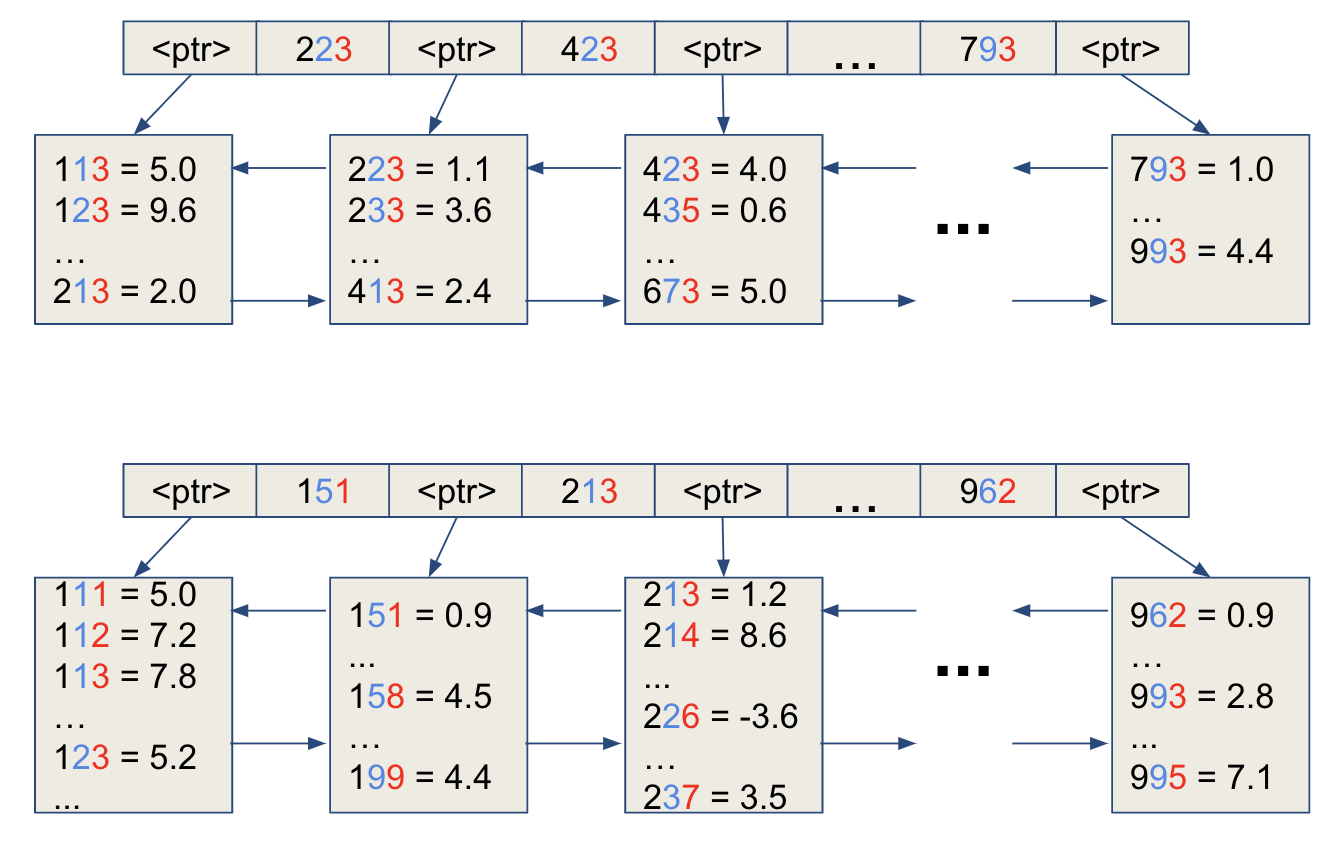
\includegraphics[scale=0.3]{update_0.png}
	\caption{Начальные значения в предикатах \lstinline{^sales} и \lstinline{sales}}
	\label{fig:optimization:random_updates:iter_init}
\end{figure}
\begin{figure}
	\centering
	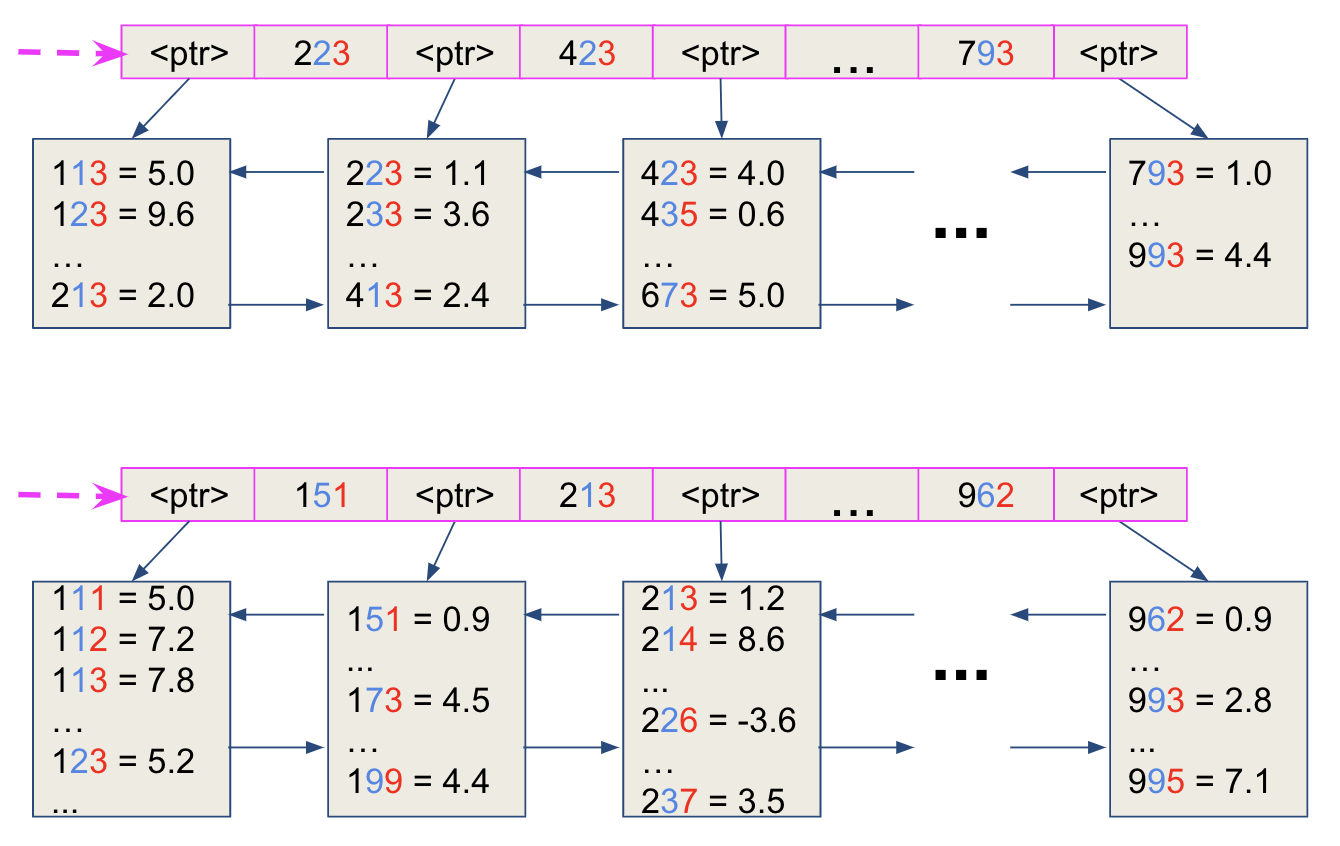
\includegraphics[scale=0.3]{update_1.png}
	\caption{Выравнивание итераторов по первым страницам}
	\label{fig:optimization:random_updates:iter_align_first}
\end{figure}
\begin{figure}
	\centering
	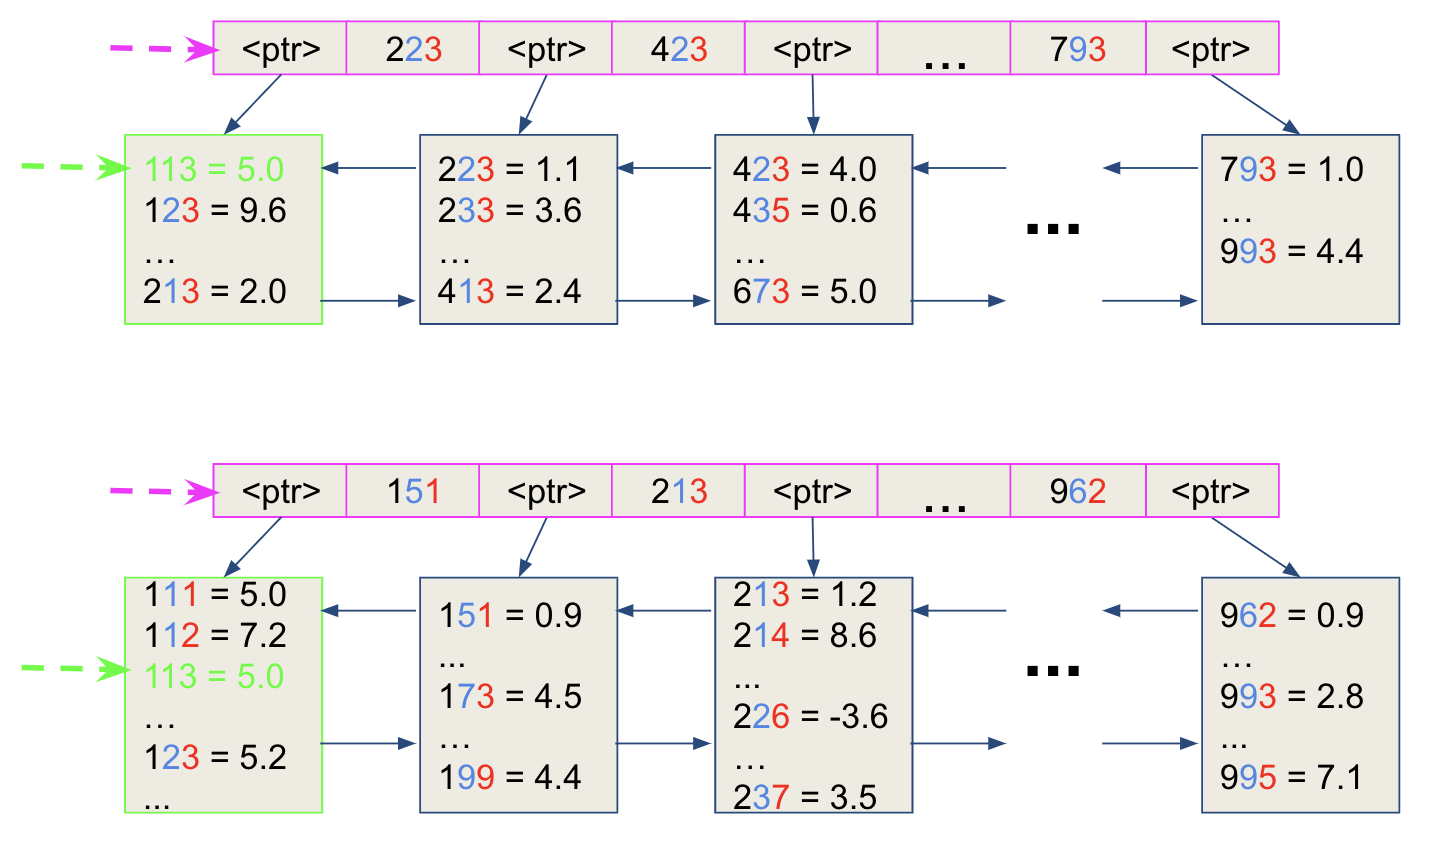
\includegraphics[scale=0.3]{update_2.png}
	\caption{Нахождение нужной записи и ее обновление}
	\label{fig:optimization:random_updates:iter_update_fact}
\end{figure}
\begin{figure}
	\centering
	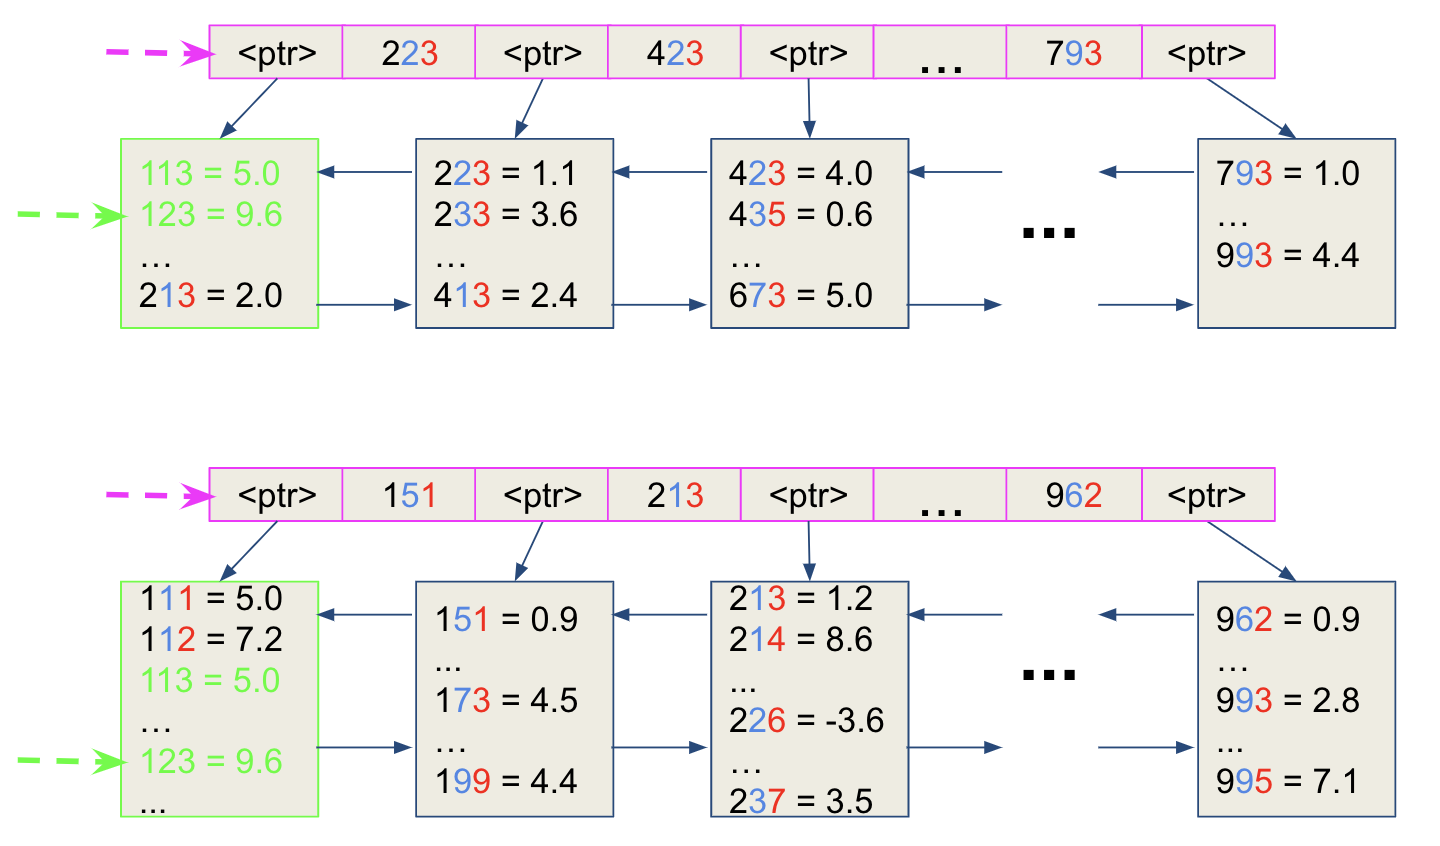
\includegraphics[scale=0.3]{update_3.png}
	\caption{Перемещение итераторов далее для обновления следующих записей}
	\label{fig:optimization:random_updates:iter_advance}
\end{figure}

Из приведенного алгоритма можно увидеть, что при обновлении пришлось пройтись \emph{по всем} страницам. Это может стать проблемой при очень больших предикатах (например, исторические данные о продажах). В таких случаях среда выполнения пытается использовать несколько итераторов, выполняя обновление параллельно (\emph{domain parallelism}). Кроме того, ситуация осложняется при операциях вставки: страницы начинают переполняться, требуя их разбиения и перезаписи. Такое происходит при разовом добавлении большого количества данных.

Разберем на примере описанную ситуацию. Пусть имеется предикат \lstinline{sales[item, location, week] = value}, который содержит историческую информацию о продажах товара в конкретном магазине в каждую неделю. По прошествии очередного интервала времени (недели) в этот предикат необходимо добавить значения о продажах за этот период. Для этого торговая сеть посылает набор файлов (\lstinline{.csv}) с такими значениями, и система начинает вносить их в базу - процесс называется \emph{batch}. В этом случае многие страницы начинают переполняться (потому что пары \lstinline{(item, location)} начинают содержать много данных), что приводит к их перераспределению. В более ранних версиях платформы эту проблему частично решало переупорядочивание ключей в предикате, делая \lstinline{sales[week, location, item] = value}, что не вызывало перезапись существующих страниц, а лишь создание новых (потому что создается новый самый первый ключ). В целом такой подход позволял ускорить время одного "батча" на $40-50\%$.
